\documentclass[11pt]{article}
\usepackage[margin=2.2cm]{geometry}
\usepackage{lmodern}
\usepackage[T1]{fontenc}
\usepackage[utf8]{inputenc}
\usepackage{graphicx,booktabs,tabularx,longtable,multirow,amsmath,amssymb,xcolor}
\usepackage[hidelinks]{hyperref}
\graphicspath{{figures/}}
\newcolumntype{Y}{>{\raggedright\arraybackslash}X}
\newcolumntype{P}[1]{>{\raggedright\arraybackslash}p{#1}}
\makeatletter
% \@@input is expandable, so generated rows can sit directly before \bottomrule.
\newcommand{\gen}[1]{\@@input generated/#1.tex }
\makeatother
\IfFileExists{generated/numbers.tex}{\newcommand{\EightWitness}{240/240}
\newcommand{\EightMotion}{113/120 (94\%)}
\newcommand{\EightCampaigns}{2}
\newcommand{\SixResult}{No drifted intent is released (0 stale releases in total). With a 500\,ms freshness window, the 5 configurations with at least 50\,ms of per-packet delay revoke every drifted intent for elapsed time rather than context, and valid controls are revoked too (50/70 over all configurations); with a 10\,s window 210/210 drifted intents are revoked on context and 70/70 controls are released. Impairment thus never makes the gate fail open, but a freshness window shorter than the transport delay turns fail-closed into denial of service.}
\newcommand{\EightCampaignsUsed}{1, 2}
\newcommand{\TenCampaigns}{5}
\newcommand{\TraceN}{500}
\newcommand{\TraceRateA}{1}
\newcommand{\TraceRateB}{10}
\newcommand{\TraceRateC}{77}
\newcommand{\TwentyPDecThirty}{2000}
\newcommand{\TwentyPObsThirty}{35}
\newcommand{\TwentyPValThirty}{1963}
\newcommand{\TwentyPDiscThirty}{2}
\newcommand{\TwentyPDecTwoForty}{2000}
\newcommand{\TwentyPObsTwoForty}{147}
\newcommand{\TwentyPValTwoForty}{1852}
\newcommand{\TwentyPDiscTwoForty}{1}
\newcommand{\TwentyPerResource}{0.13--14}
\newcommand{\EmbPiIps}{167--168}
\newcommand{\EmbVfIps}{148--152}
}{}

\title{Execution-Time Validation of Context-Carrying Action Intents:\\ Detailed Results}
\date{}
\author{Luca~D'Agati, Giuseppe~Tricomi, Fabio~Orazio~Mirto, and Giovanni~Merlino}

\begin{document}
\maketitle

\noindent This document accompanies the paper and the released artifact. It gives the protocols, the per-condition tables, and the detailed results behind every statement of the paper's evaluation. All values are generated from the frozen per-trial data in \texttt{data/execution-gap/} by \texttt{scripts/build\_detailed\_results.sh}. Experiment identifiers follow the paper; E1c denotes the valid-intent controls of E1.

\section*{1. Execution-gap failure modes}
\begin{center}\small
\begin{tabularx}{\linewidth}{@{}lYYl@{}}
\toprule
\textbf{Mode} & \textbf{Condition at release} & \textbf{Representative cause} & \textbf{Policy} \\
\midrule
Temporal obsolescence & Freshness window or deadline has elapsed & Inference, network, or queue delay & Revoke (may record \textsc{Expired}) \\
Context drift & A precondition that held at $t_d$ is false at $t_v$ or $t_g$ & Operator override or plant transition & Revoke \\
Resource conflict & Concurrent intents target the same resource & Multiple AI, vision, or human sources & Order/delay \\
Semantic fragmentation & Producers encode validity incompatibly & Middleware and application silos & Normalize in AIS \\
Unsafe delegation & A decision output is treated as authorization & Missing validation boundary & Reject before release \\
\bottomrule
\end{tabularx}
\end{center}

\section*{2. Suites and protocols}
{\small
\setlength{\LTpre}{0pt}
\setlength{\LTpost}{0pt}
\begin{longtable}{@{}P{1.85cm}P{1.30cm}P{\dimexpr\linewidth-3.15cm-4\tabcolsep\relax}@{}}
\toprule
\textbf{Suite} & \textbf{Type} & \textbf{Protocol} \\
\midrule
\endfirsthead
\toprule
\textbf{Suite} & \textbf{Type} & \textbf{Protocol (continued)} \\
\midrule
\endhead
\midrule
\multicolumn{3}{r}{\footnotesize Continued on next page} \\
\endfoot
\bottomrule
\endlastfoot
E0 & det. & Ten in-process lifecycle and contract regressions. \\
E1 & det. & Intent built at $t_d$, 200\,ms pause, PAUSED written through the gateway, submission; freshness 1000\,ms; $n{=}100$ per mode. \\
E3 & det. & AI and XR intents on one actuator at equal priority in one batch; declared tie-break. \\
E4 & perf. & 10\,000 sequential intents to the XAIR core, distinct targets. \\
E6 & fault & Stack in a network namespace, \texttt{tc netem} on its loopback; 30 drifted + 10 valid per configuration; windows 500\,ms and 10\,s. \\
E8 & sim. & E1 pattern against a headless Gazebo Harmonic cell (ROS~2 Jazzy container); ROS message witness and joint-motion witness. \\
E9 & det. & Remote write to the shared snapshot only; delay $\delta$ before submission; four policies; $n{=}10$ per cell. \\
E10 & timing & 50\,ms induced gate delay (or none, ``natural window''); invalidating write at an offset after validation; classification completed before $t_g$ / overlapping $[t_g,t_m]$ / started after $t_m$ by the gateway clock, and exact ordering by store version; optimistic release and release after an atomic authorization commit. \\
E10-ABA & timing & Line paused 10\,ms and resumed 25\,ms after submission while the gate waits 50\,ms; XAIR read-set, truth, and predicate-only gates (optimistic), read-set and truth gates (atomic), and the policy engine with and without its read-set rule; each flip trial placed by store versions; 50 flips and 25 controls per gate. \\
E10-deadline & timing & Deadline 100\,ms; induced gate delay swept 75--105\,ms in 0.5\,ms steps; ten trials per step and release path (optimistic, atomic, atomic with release guard, atomic with 3\,ms commit margin); age at the check (gateway or store clock) and at $t_m$ (shared realtime clock). \\
E11 & stoch. & Mixed valid/drifted trials, random pause, predicate count, and source; three seeds. \\
E12 & perf. & Closed loop, persistent pool of 1/10/50 producers, 1/64\,KiB snapshots, five repetitions. \\
E13 & det. & Five malformed templates, false precondition, duplicates, clock skew. \\
E14 & det. & E1 pattern for four action classes. \\
E15 & det. & Remote write carried by a local OPC~UA server. \\
E16 & perf. & 100 valid intents per condition under background writers at 0--500\,Hz; global vs.\ read-set version (single host), plus predicate-truth version and policy engine with and without its read-set rule (distributed), and global, read-set, and truth versions on the physical nodes and the embedded boards. \\
E16-trace & perf. & UCI hydraulic test rig (DOI 10.24432/C5CW21), five 60\,s cycles replayed without interruption as OPC~UA-style notifications (deadband 0) at 1000/100/10\,ms; the 1200 intents of each interval (twelve cells, $n{=}100$) are interleaved at random and spread uniformly over the 300\,s replay with a random phase; discrete and continuous intents; global, read-set, predicate-truth, and predicate-only scope, and the policy engine with and without its read-set rule. \\
E17 & det. & Producer omits the line-state precondition; drift and valid trials with and without a server-side policy; $n{=}100$ per cell. \\
E18 & fault & Actuation log against the store: gateway crash after commit, retried commit, consumer crash between effect and offset update, consumer restarts, concurrent committers, read-set change after commit; 10 repetitions of 100 commits. \\
E18b & fault & Store with append-only file fsynced on every write; committer and consumer killed with SIGKILL and restarted, store killed and restarted twice per run; SQLite-backed idempotent actuator; five runs of 1000 commits. \\
E20 & trace & Job-shop event log (4TU, 89 days, 31 resources): offline drift prevalence for latencies 1\,s--1\,h, exact over the timeline (one-minute timestamps), under three decision models (uniform over idle time, idle intervals of at most 8\,h, one decision at the start of each idle interval) and three invalidation proxies (the machine leaves idle, the next step is for a different part, the next step is a breakdown), with a Monte Carlo cross-check; live replay of 30 days at 8640$\times$, START\_JOB on idle machines after 30 or 240 plant minutes, five gates, decisions assigned to gates in rotation (200 per gate and latency). \\
E21 & timing & OPC~UA cell controller owning the line state (10\,ms scan, asynchronous mirror to XAIR); operator pause at the controller 0--30\,ms after submission; unconditional command, controller-local interlock (executed only on a running line), and version-conditional command, optimistic and atomic; 20 injected trials per offset and path, 20 controls. E21-ABA: pauses 0--20\,ms after submission, each followed by a resume 3\,ms later (10\,ms on the LAN, 20\,ms over the wide-area overlay); an execution on a running line at a controller version newer than the one the check observed is a history violation. \\
E22 & physical & Gateway and cell controller on a separate machine (Apple M4). Wide area (TCP connect 62\,ms): E1, E1c, E10 natural window, E10-ABA (flip at 280/450\,ms, gate delay 400\,ms; on both physical nodes each flip trial is placed by store versions and repeated until every gate has 50 trials whose flip falls between validation and the check), E16 (0--20\,Hz), E21 (pauses 0--200\,ms) and E21-ABA (pauses 80--200\,ms). Wi-Fi LAN (TCP connect 6.6\,ms median), with XAIR, Redis, and the producers on a Raspberry Pi~4: the same suites, E10-ABA with flip at 80/130\,ms and gate delay 200\,ms, E16 (0--100\,Hz), E21 (pauses 0--120\,ms) and E21-ABA (pauses 0--80\,ms). \\
E23 & scale & Dedicated store; 0--10\,000 registered predicates on as many paths; updates changing 0--100\% of those paths (truth preserved); document vs.\ hash layout; update latency and throughput, validation read, registry size, store memory; retirement with a short retention. \\
E24 & PLC & OpenPLC~v3 runtime, Structured Text program in a 10\,ms task owning the line state and its version (unconditional, interlock on the line state, or version-conditional; no deadline check in the PLC); Modbus~TCP; poller replicating the state to XAIR every 5\,ms; E21 protocol with pauses 0--100\,ms after submission. \\
E25 & embedded & Raspberry Pi~4 (Cortex-A72, PREEMPT\_RT) and VisionFive~2 (SiFive U74, RISC-V); Redis (container on the Pi, built from source on the VisionFive), XAIR, gateway, and harness each pinned to one core, loopback; E4 (three runs of 3000 intents), E11 (three seeds), E10 natural window (both modes), E16 (0--100\,Hz; global, read-set, truth). \\
\end{longtable}}

\section*{3. E16 context churn (full)}
Target and achieved writer rates, false positives, goodput, and end-to-end p99.
\begin{center}\small
\footnotesize\setlength{\tabcolsep}{3.5pt}
\begin{tabular}{@{}llrrcrr@{}}
\toprule
\textbf{Scope} & \textbf{Pattern} & \textbf{Target [Hz]} & \textbf{Achieved [Hz]} & \textbf{Revoked} & \textbf{Goodput [1/s]} & \textbf{E2E p99 [ms]} \\
\midrule
\gen{tab_e16}
\bottomrule
\end{tabular}
\end{center}
\begin{center}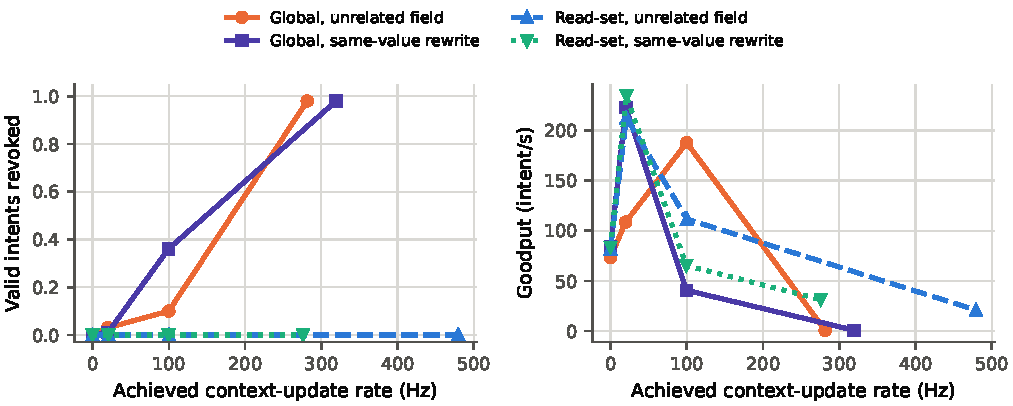
\includegraphics[width=0.85\linewidth]{e16_context_churn.pdf}\end{center}
\noindent Single-host campaign: false revocations (left) and goodput of valid intents (right) against the achieved update rate. Read-set versions revoke none.

\section*{4. E6 network impairment}
Delay/jitter/loss [ms/ms/\%], median end-to-end latency, stale releases, revocation reasons of drifted intents, and valid controls released.
\begin{center}\small
\begin{tabular}{@{}lrcccll@{}}
\toprule
& & \multicolumn{3}{c}{\textbf{Window 500\,ms}} & \multicolumn{2}{c}{\textbf{Window 10\,s}} \\
\cmidrule(lr){3-5}\cmidrule(lr){6-7}
\textbf{Impairment} & \textbf{E2E p50 [ms]} & \textbf{Stale} & \textbf{Reasons} & \textbf{Valid rel.} & \textbf{Reasons} & \textbf{Valid rel.} \\
\midrule
\gen{tab_e6}
\bottomrule
\end{tabular}
\end{center}

\section*{5. E8-Gazebo per campaign, E15, E3, and E0}
Released, ROS messages observed, ROS-witness agreement, and joint motion per mode. Campaigns whose ROS subscriber stalled are listed but excluded from the witness figures of the paper.
\begin{center}\small
\begin{tabular}{@{}llcccc@{}}
\toprule
\textbf{Campaign} & \textbf{Mode} & \textbf{Released} & \textbf{ROS msgs} & \textbf{Witness agrees} & \textbf{Motion} \\
\midrule
\gen{tab_e8}
\bottomrule
\end{tabular}
\end{center}
\noindent The joint-motion tracker never reports motion without a release and detects \EightMotion\ releases. Each of the seven misses had zero joint displacement although the command was observed, consistent with an arm already at the commanded pose; the tracker is therefore a conservative proxy, and the message-level witness the reliable one. E14 repeats the E1 pattern for \texttt{STOP}, \texttt{GRASP}, and \texttt{SET\_SPEED} (100/100 vs.\ 0/100 per condition); E15 carries the remote write over OPC~UA (stale and un-notified push caches 30/30, XAIR 0/30); E13 passes 250/250 declared cases; E3 confirms the declared tie-break (100/100); E0 passes ten lifecycle regressions.

\section*{6. E14 action classes and E13 fault cases}
\begin{center}\small
\begin{tabular}{@{}lccc@{}}
\toprule
\textbf{Scenario} & \textbf{Direct} & \textbf{Local} & \textbf{XAIR} \\
\midrule
\gen{tab_e14}
\bottomrule
\end{tabular}
\qquad
\begin{tabular}{@{}lc@{}}
\toprule
\textbf{Fault} & \textbf{Passed} \\
\midrule
\gen{tab_e13}
\bottomrule
\end{tabular}
\end{center}

\section*{7. E11 validation cost by conjunction length (valid trials)}
\begin{center}\small
\begin{tabular}{@{}rrrrr@{}}
\toprule
\textbf{Predicates} & \textbf{$n$} & \textbf{p50 [ms]} & \textbf{p95 [ms]} & \textbf{max [ms]} \\
\midrule
\gen{tab_e11_cost}
\bottomrule
\end{tabular}
\end{center}

\section*{8. Single-host E10}
Shared host, optimistic release, 50\,ms induced gate delay ($n{=}30$ per offset); position of each write by the gateway clock (released in parentheses).
\begin{center}\small
\begin{tabular}{@{}rcccc@{}}
\toprule
\textbf{Offset [ms]} & \textbf{Before $t_g$} & \textbf{Overlapping $[t_g,t_m]$} & \textbf{After $t_m$} & \textbf{Released} \\
\midrule
0--30 & 180 (0) & 0 (--)  & 0 (--)   & 0/180 \\
40  & 29 (0) & 1 (0)   & 0 (--)   & 0/30 \\
45  & 12 (0) & 18 (4)  & 0 (--)   & 4/30 \\
50  & 0 (--) & 28 (18) & 2 (2)    & 20/30 \\
55  & 0 (--) & 17 (16) & 13 (13)  & 29/30 \\
60, 100 & 0 (--) & 0 (--) & 60 (60) & 60/60 \\
\bottomrule
\end{tabular}
\end{center}
\begin{center}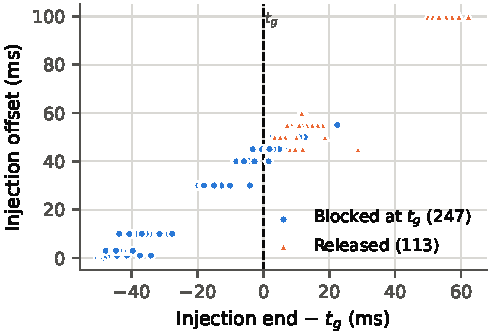
\includegraphics[width=0.75\linewidth]{e10_injection_timing.pdf}\end{center}
\noindent End of the invalidating write relative to $t_g$ for every injected single-host trial. Gateway-side residual interval, from the end of the recheck to the middleware call: 0.012/0.037/0.200\,ms (p50/p99/max over 183 releases); recheck round trip 2.4\,ms median.

\section*{9. E12 scaling in the three configurations}
Median over five repetitions; 500/500 released and no connection retries in every condition. Throughput [intent/s] / p50 / p99 [ms].
\begin{center}\small
\begin{tabular}{@{}rrcccc@{}}
\toprule
& & \multicolumn{2}{c}{\textbf{Reserved cores}} & \multicolumn{2}{c}{\textbf{Distributed testbed}} \\
\cmidrule(lr){3-4}\cmidrule(lr){5-6}
\textbf{Producers} & \textbf{KiB} & \textbf{Local auth.} & \textbf{XAIR} & \textbf{Local auth.} & \textbf{XAIR} \\
\midrule
\gen{tab_e12_both}
\bottomrule
\end{tabular}
\end{center}
Shared host (load average 68--75), for comparison:
\begin{center}\small
\begin{tabular}{@{}rrcc@{}}
\toprule
\textbf{Producers} & \textbf{KiB} & \textbf{Local auth.} & \textbf{XAIR} \\
\midrule
1  & 1  & 348 / 2.8 / 3.7     & 99 / 9.1 / 23.6 \\
1  & 64 & 97 / 9.7 / 21.1     & 85 / 11.2 / 27.5 \\
10 & 1  & 299 / 31.8 / 53.0   & 436 / 22.1 / 29.0 \\
10 & 64 & 200 / 46.8 / 69.4   & 332 / 28.8 / 45.2 \\
50 & 1  & 663 / 59.1 / 74.0   & 193 / 201.4 / 272.0 \\
50 & 64 & 419 / 100.2 / 134.4 & 174 / 218.0 / 326.9 \\
\bottomrule
\end{tabular}
\end{center}
E4 on reserved cores (three runs of 10\,000 intents): \gen{tab_e4_reps}

\section*{10. E16 on the distributed testbed}
\begin{center}\small
\footnotesize\setlength{\tabcolsep}{3.5pt}
\begin{tabular}{@{}llrrcrr@{}}
\toprule
\textbf{Scope} & \textbf{Pattern} & \textbf{Target [Hz]} & \textbf{Achieved [Hz]} & \textbf{Revoked} & \textbf{Goodput [1/s]} & \textbf{E2E p99 [ms]} \\
\midrule
\gen{tab_e16_dist}
\bottomrule
\end{tabular}
\end{center}
\noindent Campaign 1 of the distributed testbed. Distributed E1 and E9 reproduce the single-host counts exactly (direct and freshness-only 100/100, contextual policies 0/100, FPR 0/100; E9 60/60, 20/60, 0/60, 0/60). Across the five campaigns, the global-version rates for the unrelated-field pattern are 9--12\% at 20\,Hz and 58--68\% at 100\,Hz, and read-set and predicate-truth versions and the policy engine, with or without its read-set rule, revoke 0/100 in all of their cells. Sensitivity: with $2\pm1$\,ms of delay per interface, the natural-window validation-to-release median rises to 13.6\,ms (optimistic) and 14.7\,ms (atomic), the check-to-$t_m$ bounds to 2.5--6.8 and 2.4--6.8\,ms, and the global version revokes 95--99\% at 100\,Hz; with CPU sets shared by all components, the natural-window figures stay within 0.2\,ms of the baseline and the global version revokes 79--82\% at 100\,Hz; in both variants no release followed a write committed before its check or before $t_m$. Testbed: containers on disjoint CPU sets, $0.5\pm0.1$\,ms of shaped delay per interface, TCP connect 1.2--1.3\,ms median; the store-side monotonic timestamps fell inside the requesting interval in 50/50 checks at the start of every campaign.

\section*{11. Distributed testbed: per-offset E10, policy, and faults}
Campaign 1, per offset (30 injected writes per offset and mode). Clock position of the optimistic trials by the gateway clock alone (completed before $t_g$ / overlapping $[t_g,t_m]$ / started after $t_m$); ``potential'': optimistic releases whose write overlapped $[t_g,t_m]$ on that clock; ``stale'': releases after an atomic commit although the write was ordered before the commit by store version, which a correct commit refuses.
\begin{center}\small
\begin{tabular}{@{}rccccc@{}}
\toprule
\textbf{Offset [ms]} & \textbf{Clock position} & \textbf{Opt.\ released} & \textbf{Potential} & \textbf{Atomic released} & \textbf{Stale} \\
\midrule
\gen{tab_e10_modes}
\bottomrule
\end{tabular}
\end{center}
\gen{tab_dist_extra}

\section*{12. Additional figures}
\begin{center}
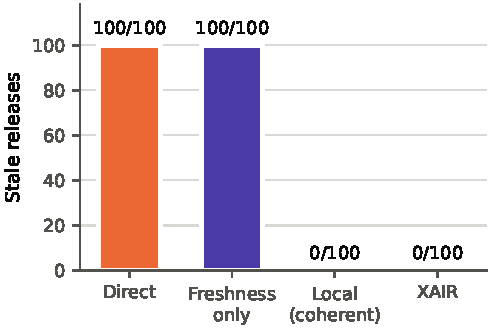
\includegraphics[width=0.45\linewidth]{e1_ser_by_baseline.pdf}\hfill
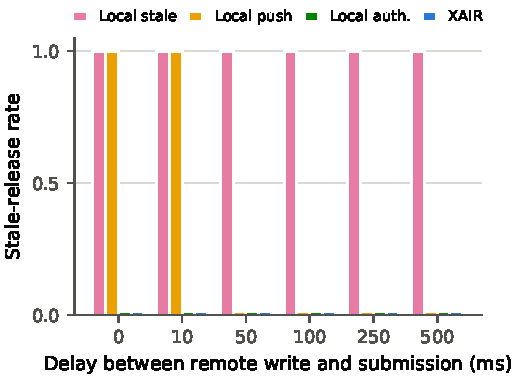
\includegraphics[width=0.45\linewidth]{e9_consistency_sweep.pdf}\\[1ex]
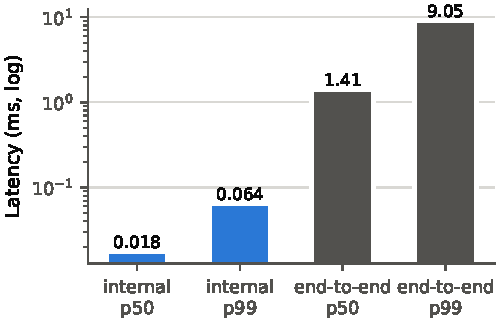
\includegraphics[width=0.45\linewidth]{e4_load_latency.pdf}\hfill
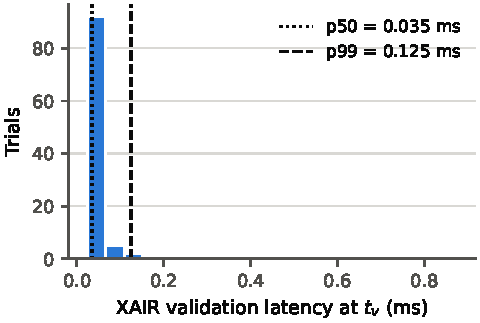
\includegraphics[width=0.45\linewidth]{e1_validation_latency.pdf}
\end{center}
\noindent Single-host campaign (S), whose latencies are orders of magnitude only: E1 stale releases by mode (100 obsolete intents each); E9 stale-release rate by policy and delay ($n{=}10$ per bar; bars at zero are not drawn); E4 internal vs.\ end-to-end latency (log scale); E1 XAIR validation latency. The paper's performance figures come from the reserved-core and embedded configurations.

\section*{13. E1 per testbed}
E1: obsolete \texttt{RESUME} released / trials, and median end-to-end latency [ms], per testbed ($n{=}100$ per mode; $0/100$ has 95\% upper bound 0.037).
\begin{center}
\small
\begin{tabular}{@{}lcccc@{}}
\toprule
\textbf{Mode} & \textbf{Single host} & \textbf{Distributed} & \textbf{Physical, wide area} & \textbf{Physical, Wi-Fi LAN} \\
\midrule
\gen{tab_e1_all}
\bottomrule
\end{tabular}
\end{center}

\section*{14. E23 scaling of predicate-truth versions}
When an update touches none of the registered paths, it takes 7.0--13\,ms in the document layout with 1000 predicates against 1.9--6.0\,ms without, and 60--82\,ms with 10\,000 (ranges over repetitions). In the hash layout it costs no more than without predicates from 1000 predicates on, while an update touching most of them costs more than in the document layout (31--36 against 14--20\,ms with 1000). Retirement with a short retention returned 1000 unused predicates to one.

E23: cost of predicate-truth versions ($n$ predicates on $n$ paths; share of paths changed per update, truth preserved; three repetitions). Update median (range over repetitions) and maximum [ms], observations, updates/s, validation read [ms], size [KiB], and update median without predicates (range over repetitions) [ms].
\begin{center}
\footnotesize
\setlength{\tabcolsep}{3.5pt}
\begin{tabular}{@{}rlrrrrrrrr@{}}
\toprule
$n$ & \textbf{Layout} & \textbf{Chg. [\%]} & \textbf{Update} & \textbf{Max} & \textbf{Obs.} & \textbf{Upd./s} & \textbf{Valid.} & \textbf{KiB} & \textbf{No preds} \\
\midrule
\gen{tab_e23}
\bottomrule
\end{tabular}
\end{center}

\section*{15. E21, E22, and E24 by pause offset}
Stale effects [\%] of unconditional commands (optimistic release) by the offset of the pause after submission [ms], as offset: rate. A pause before XAIR's check is blocked, a pause after the effect is harmless, and only pauses in between, a window set by the replication and transport delays, act on a paused line; the pooled rates of the paper depend on how many offsets fall in that window.
\begin{center}\small
\begin{tabularx}{\linewidth}{@{}lX@{}}
\toprule
\textbf{Testbed} & \textbf{Offset [ms]: stale effects [\%]} \\
\midrule
\gen{tab_e21_offsets}
\bottomrule
\end{tabularx}
\end{center}

\section*{16. E10-deadline}
Sweeping the gateway's delay across a 100\,ms deadline (table below), no release was admitted with an age above the deadline at its check. The check is the gateway's temporal test after its store read returns (optimistic) or the commit $t_c$ (atomic), so the optimistic check-to-$t_m$ interval (0.04\,ms) excludes the return trip that $\Delta_r$ in E10 includes. At $t_m$, 193 of 1387 atomic releases (13.9\%) were late, because $t_m$ follows the commit by about 1.8\,ms; a release guard leaves 4 of 1210 and a 3\,ms commit margin none of 1097, against 5 of 1237 for the optimistic gate.

\noindent E10-deadline: releases whose age exceeded the 100\,ms deadline at the check or at the middleware call, and median check-to-$t_m$ interval (five campaigns). Late counts are out of released intents.
\begin{center}
\footnotesize
\setlength{\tabcolsep}{4pt}
\begin{tabular}{@{}lrrrrc@{}}
\toprule
\textbf{Release path} & \textbf{Trials} & \textbf{Released} & \textbf{Late, check} & \textbf{Late, $t_m$} & \textbf{Check$\to t_m$ [ms]} \\
\midrule
\gen{tab_e10_deadline}
\bottomrule
\end{tabular}
\end{center}

\section*{17. Detailed results}
The paper states each result with its decisive figures. Arrival models (Discussion): with mean gate latencies, and excluding cells where the writers saturate and contend with the gate, the better of the Poisson and periodic forms matches the single-host, distributed, trace, wide-area, and LAN cells within 3.5, 6.2, 6.2, 4.0, and 6.7 percentage points; on the embedded boards the periodic form is within 13 points and the Poisson form underestimates by up to 41. An undetected change in the optimistic interval has probability $\lambda_R\Delta_r$, i.e.\ $1$--$2\cdot10^{-3}$ per release on the distributed testbed and $2$--$4\cdot10^{-3}$ on the embedded boards for one change per second. This section gives the full account, with every count, range, and testbed detail, in the order of the paper.

\paragraph{Testbeds}
All components run on Python~3.12 with FastAPI and Redis~7.4, on six testbeds. The \emph{single-host} configuration (S) runs every suite on loopback of a shared AMD EPYC~7313 host (load average 68--75); its latencies are orders of magnitude only, and the performance figures below come from the other configurations, except the per-predicate cost of E11. The \emph{distributed} configuration (D) places Redis, the policy engine, XAIR, the gateway, an emulated cell controller, and the producers in containers with disjoint CPU sets and $0.5\pm0.1$\,ms of shaped delay per interface. It hosts five campaigns and three sensitivity variants ($2\pm1$\,ms delay, shared CPU sets, phase-locked replay), and its containers share one monotonic clock, verified at the start of every campaign. A \emph{reserved-core} configuration (R) repeats E4 and E12. Two \emph{physical} testbeds move the gateway and the controller to a separate machine (Apple M4), where only store versions order events. On the \emph{wide-area node} (P; TCP connect 62\,ms median), XAIR, Redis, and the producers stay on the EPYC host; on the \emph{LAN node} (L; Wi-Fi, TCP connect 6.6--6.8\,ms median, 10.7--14.5\,ms p99 in its two runs), they run on a Raspberry Pi~4. E22 denotes the suites repeated on P and L. On the \emph{embedded} testbed (B; E25), Redis, XAIR, the gateway, and the harness run on one edge board, each pinned to its own core: a Raspberry Pi~4 (Cortex-A72, PREEMPT\_RT kernel) and a VisionFive~2 (SiFive U74, RISC-V). The OpenPLC runtime of E24 and the dedicated store of E23 run in containers on the EPYC host.

\paragraph{Stale actuation and operator policy (RQ1: E1, E14, E8, E17)}
With $n{=}100$ per mode, a 200\,ms pause, and a 1000\,ms freshness window, both floors release every obsolete \texttt{RESUME} and every contextual policy releases none, on the four testbeds and, for the policy engine, on the distributed testbed (Section~13). Valid controls are released 100/100. The pattern holds for three further action classes (E14) and in a simulated Gazebo cell under ROS~2, where an independent subscriber on the actuator topic agrees with the gateway on \EightWitness\ trials (E8). In E17, a \texttt{RESUME} that declares only the gripper state is released after a pause in 100/100 trials, since XAIR checks what the producer declared; with an operator policy that makes the line state mandatory, 0/100 are released, and valid controls remain 100/100.

\paragraph{Consistency class (RQ2: E9, E15)}
In E9 a remote writer updates only the shared snapshot and the intent is submitted 0--500\,ms later. The never-refreshed cache releases 60/60 obsolete intents, read-through and XAIR 0/60, and the push policy exactly the 20 trials submitted before its notification, on both testbeds; the delay matters only for the push policy, so E9 establishes the consistency ladder, not a propagation curve. Carrying the write over OPC~UA reproduces it (E15).

\paragraph{Optimistic recheck and atomic commit (RQ3: E10)}
A recheck before release blocked every write ordered before it, but leaves an interval of 0.9--2.3\,ms before the middleware call. A thread writes an invalidating update at a controlled offset after validation, while the gateway waits an induced 50\,ms before its check or with no induced delay. Each write is ordered exactly against the check, by the global version it created, and located against $t_m$ by shared-clock bounds on its commit (the corresponding table of the paper; 30 writes and 10 controls per offset and campaign). In both modes all 1551 writes ordered before the check were blocked. No injected write landed in the interval between the check and $t_m$: the writes take a network round trip to commit, and the interval is short. $\Delta_r$ lies between 1.0 and 2.2\,ms at the median, and $(t_c,t_m]$ between 0.9 and 2.3\,ms. E10 therefore measures the width of the interval, not its rate of stale releases; that changes in it do reach the actuator is shown at the controller, where the replica lags by more (E21). On the gateway clock alone, 463 of the 879 optimistic releases could only have been classified as potentially stale; store versions and the shared clock resolve all of them. The atomic commit adds no measurable validation-to-release latency (4.3--4.5\,ms in either mode, without the induced delay), because one request replaces the gate's snapshot read. On the physical nodes validation to release takes 124--125\,ms on the wide-area node and 15\,ms on the LAN node, and every write ordered before the check was blocked. Without a shared clock, a write between the check and $t_m$ cannot be located there, so these nodes test only the ordering against the check. On the embedded boards (E25), which share one clock, the interval is 2.0--3.6\,ms (Raspberry Pi~4) and 2.4--4.2\,ms (VisionFive~2) at the median; no released write was committed before $t_m$, and 6 of 174 overlapped it on the VisionFive~2.

\paragraph{Deadline at release (RQ3: E10-deadline)}
No release was admitted with an age above the deadline at its check. At $t_m$, 193 of 1387 atomic releases (13.9\%) were late, because $t_m$ follows the commit by about 1.8\,ms; a release guard or a 3\,ms commit margin keeps the deadline at $t_m$ (4 of 1210 and 0 of 1097 late, against 5 of 1237 for the optimistic gate; Section~16).

\paragraph{History violations undone before the check (RQ3: E10-ABA)}
While the gateway waits, the harness pauses the line and resumes it before the check, so every predicate holds at the check although it was false in the interim (the corresponding table of the paper). These are history violations, not stale releases under the pointwise definition of the paper. Each trial is placed by store versions and tests a history violation only if both writes fall between the validation snapshot and the check; on the distributed testbed all did. Read-set and predicate-truth versions block every such intent in both modes, and so does the policy engine once its rule compares the read-set version it computes from the replicated per-path versions; the predicate-only gate and the policy engine without versions release 250/250. Versioning is therefore a property of the check, not of the runtime that performs it. On the physical nodes, trials are repeated until every gate has 50 trials inside the window; the versioned gates release 0/50 on both nodes and the predicate-only gate 50/50. In 11 wide-area trials and 1 LAN trial, validation came after the pause; they are excluded.

\paragraph{The last check at the controller (RQ3: E21)}
A check on XAIR's copy lets about half of the unconditional commands act on a paused line; any check in the controller's scan removes these effects. In E21 an emulated OPC~UA cell controller owns the line state, executes commands at its 10\,ms scan, and replicates its state to XAIR asynchronously. An operator pause is written at the controller 0--30\,ms after submission, and ground truth is the controller's state at the effect (the corresponding table of the paper). Three ways of handing the command to the controller follow XAIR's check, in either release mode: an unconditional command, a controller-local interlock that executes only on a running line, and a command conditional on the controller's version as the check observed it. With unconditional commands, 567 and 569 of 1100 injected trials took effect on a paused line (48--54\% per campaign), because XAIR's copy lags the controller. The rate is not a property of the system but of where the pauses fall (Fig.~4d of the paper; Section~15): a pause written up to 2\,ms after submission reaches XAIR before its check and is blocked, one written 6--12\,ms after escapes the check in 94--100\% of trials (optimistic release; 92--100\% atomic), and at 20 and 30\,ms it comes after the effect in 90 and 100\% of trials. The unprotected window thus spans about 4--20\,ms on this testbed, 20--80\,ms on the LAN, and from about 160\,ms on over the wide-area overlay, and its position follows the replication and transport delays of each configuration. Both controller-side paths remove stale effects, as their construction implies: the interlock refused 556 and 581 commands and the conditional command 576 and 571, and every valid control executed.

The two differ when the pause is followed, 3\,ms later, by a resume (E21-ABA). The interlock then finds a running line and executes: 285 and 297 of 1000 trials took effect after a change that was undone between the check and the effect, a history violation on the controller's state. The version-conditional command refused all of them, as the version had advanced, and produced neither a stale effect nor a history violation. On the physical nodes the pattern repeats for pauses (42 and 37 of 180 stale effects on the wide-area node, 44 and 51 on the LAN node, none for the interlock or the version-conditional command). Pause--resume pairs rarely fit between the check and the effect there, and the interlock let 1--3 of 140 through against none for the conditional command.

\paragraph{The last check on a PLC runtime (RQ3: E24)}
A PLC runtime reproduces E21: unconditional commands acted on a paused line, while the interlock and the version-conditional command never did. E24 repeats E21 on an OpenPLC~v3 runtime executing a Structured Text program in a 10\,ms task, reached over Modbus, with a poller replicating its state to XAIR every 5\,ms (the corresponding table of the paper). Unconditional commands took effect on a paused line in 30/180 and 29/180 trials, all but one with the pause scheduled at most 10\,ms after submission (all written within 30\,ms); the interlock and the version-conditional command in none, the PLC refusing 34--38 per path. The atomicity of check and effect comes from the runtime's scan cycle. The program checks only the version: its 16-bit registers carry no absolute time, so in E24 the deadline holds at the gateway's check or the commit, not in the scan (the E21 controller checks both). Its 16-bit version changes at most once per scan, so a value cannot recur within about 327\,s at the nominal period, far longer than any trial's span from the replica read to the effect. The runtime runs in a container, and the effect is a register write, not physical output.

\paragraph{Version scope under churn (RQ4: E16, E16-trace)}
Only a global version turns unrelated updates into revocations, and more so the slower the gate. E16 submits 100 valid intents per condition while background writers update the snapshot at 0--500\,Hz, changing an unrelated field or rewriting the line state with its current value, so every revocation is a false positive (the corresponding table of the paper). A global version revokes 12\% of valid intents at 20\,Hz, 64\% at 100\,Hz (62--70\% per campaign), and 99.5\% (99--100\% per campaign) once writers saturate near 120\,Hz; read-set and predicate-truth versions and the policy engine, with or without its read-set rule, revoke none. The global rate grows with the gate latency on every testbed: 10--36\% at 100\,Hz on the faster single host, 94--99\% on the embedded boards (gate 5--10\,ms), all at 100\,Hz on the LAN node (about 35\,ms), and 96--98\% already at 5\,Hz on the wide-area node (over 120\,ms); read-set and truth versions revoke none on any of them (Section~10).

On a recorded trace, read-set versions still revoke continuous intents whose signal changes value constantly; predicate-truth versions do not. E16-trace replays five 60\,s cycles of a public hydraulic test-rig recording~ (17 sensors at 1--100\,Hz) as the notifications of an OPC~UA subscription with zero deadband at 1000, 100, or 10\,ms. Discrete intents read only the line and gripper state, which the trace never writes; continuous intents also require a 100\,Hz pressure to stay below 250\,bar, which it always does (the corresponding table of the paper). Read-set versions remove false revocations for discrete intents but not for continuous ones: the pressure changes value in almost every notification, so at 10\,ms 37\% of valid continuous intents are revoked (34--41\% per campaign), as many as under a global version, and 26\% with the policy engine's read-set rule, whose gate is faster. Predicate-truth versions remove them, since the threshold is never crossed, as do the gates without versions. With a phase-locked submission the 10\,ms rates are similar (37\% read-set).

\paragraph{Prevalence in a production log (RQ4: E20)}
In a production log, drift within a minute is rare unless decisions are taken the moment a machine becomes idle; for decisions that wait tens of minutes it ranges from a few percent to a large share, depending on how the plant schedules (the corresponding table of the paper). E20 uses the event log of a job shop~ (4543 work steps on 31 resources over 89 days, one-minute timestamps). With decisions spread uniformly over the idle time between recorded steps, the machine leaves the idle state within a decision-to-release latency $\ell$ for 0.13\% of decisions at 1\,min, 3.0\% at 30\,min, and 5.4\% at 1\,h (0.08, 1.7, and 3.1\% if the idle time before each machine's first and after its last step, which the log does not describe, is included). Without idle intervals longer than 8\,h, mostly nights and weekends, the fractions rise to 19 and 32\% at 30\,min and 1\,h (under 1\% at 1\,min); a scheduler that decides as soon as a machine becomes idle sees 35 and 43\% (14\% at 1\,min, a figure bounded by the log's resolution). Narrower proxies give 1.1--9.8\% at 30\,min to 1\,h when the next step is for a different part, and at most 1.1\% when it is a breakdown; across resources, the uniform fraction at 1\,h ranges over \TwentyPerResource\%. In a live replay of 30 days, 8640 times faster, a scheduler starts jobs on idle machines after 30 or 240 plant minutes, and decisions go to the five gates in rotation (200 per gate and latency). The direct floor released all 18 of its obsolete decisions and the XAIR gates none of 62; the global version also revoked 5/195 and 6/191 valid decisions, the read-set and truth versions none of 1152. With so few per cell, the replay shows that the gates behave on the log as in the controlled suites, not how their rates compare.

\paragraph{Cost on edge processors (RQ5: E25)}
On both boards, with each process pinned to one core and everything on loopback (the corresponding table of the paper), XAIR validates \EmbPiIps\ (Raspberry Pi~4) and \EmbVfIps\ (VisionFive~2) sequential intents/s, a fifth to a sixth of the reserved EPYC cores below. Internal validation takes 0.10--0.13\,ms and the end-to-end path 5.7--6.4\,ms at the median. Predicate cost grows from 0.11--0.16\,ms for 2 predicates to 0.28--0.68\,ms for 32. Validation to release takes 5.0--6.2\,ms in either release mode. The slower gate raises the cost of a global version, as E16 showed: 94--99\% of valid intents are revoked at 100\,Hz, against 64\% on the distributed testbed, while read-set and truth versions revoke none. XAIR's resident memory is 93--96\,MB, most of it the Python runtime.

\paragraph{Cost, scaling, and faults (RQ5: E4, E11, E12, E18, E6)}
On reserved cores XAIR validates 909--956 sequential intents/s, with 0.017--0.018\,ms internal and about 1.0\,ms end-to-end median latency. On the single host, predicate cost grows from 0.039\,ms for 2 predicates to 0.115\,ms for 32 (E11). In closed loops of 1--50 producers (E12), every condition releases 500/500; on reserved cores read-through has a 1.2--1.9$\times$ lower median latency than XAIR, as its one fewer exchange predicts, and on the distributed testbed a similar throughput. The policy-engine path is faster still (99--600 against 54--249 intents/s on the distributed testbed) but does less per intent: two small queries on in-memory data, with no lifecycle, idempotency, or release records, and no store read. Its data are replicated by XAIR's write path, which E12 does not load. The actuation log lost no command and produced no second effect under emulated crashes (E18) and under real ones (E18b: 5000 commits, with the committer, the consumer, and the store killed abruptly 14, 43, and 10 times). This does not show exactly-once physical effects: an actuator whose motion and record are not one atomic step can crash between them. Under network impairment no drifted intent was released, but a 500\,ms window shorter than the transport delay revoked 50/70 valid controls (E6); regression suites for malformed inputs, tie-breaks, and the lifecycle pass (E13, E3, E0).

\paragraph{Scaling of predicate-truth versions (RQ5: E23)}
With a single writer, predicate-truth versions sustain about 100 updates/s up to about a thousand registered predicates when updates touch a small share of them (E23; three repetitions on a loaded host). An update that touches none of them costs 7.0--13\,ms in the document layout with 1000 predicates against 1.9--6.0\,ms without, and no more than without predicates in the hash layout; layouts, retirement, and timings up to 10\,000 predicates are in Section~14.

\section*{18. Tables summarized in the paper}
The paper states these results in its text and in its key-results figure; the full tables follow.

\noindent E10 on the distributed testbed, pooled over five campaigns: injected writes relative to the check (store version) and to $t_m$ (shared clock); interval rows: natural window, ranges of per-campaign medians. Controls: 400/400 and 150/150 released per mode.
\begin{center}\small\setlength{\tabcolsep}{3pt}
\begin{tabular}{@{}llcc@{}}
\toprule
\textbf{Window} & & \textbf{Optimistic} & \textbf{Atomic} \\
\midrule
\gen{tab_e10_summary}
\bottomrule
\end{tabular}
\end{center}

\noindent E16: valid intents revoked [\%] under synthetic context updates, by gate (1000 per condition: two patterns, five campaigns; the highest target rate reached about 120\,Hz).
\begin{center}\small
\begin{tabular}{@{}lccc@{}}
\toprule
\textbf{Gate} & \textbf{20\,Hz} & \textbf{100\,Hz} & \textbf{500\,Hz target} \\
\midrule
\gen{tab_e16_pooled}
\bottomrule
\end{tabular}
\end{center}

\noindent E16-trace: valid intents revoked [\%] while a recorded hydraulic test rig is replayed as context updates, by gate and publishing interval (500 per condition over five campaigns; about \TraceRateA, \TraceRateB, and \TraceRateC\ updates/s; disc.: discrete, cont.: continuous intent).
\begin{center}\small\setlength{\tabcolsep}{4pt}
\begin{tabular}{@{}lcccccc@{}}
\toprule
& \multicolumn{2}{c}{\textbf{1000\,ms}} & \multicolumn{2}{c}{\textbf{100\,ms}} & \multicolumn{2}{c}{\textbf{10\,ms}} \\
\cmidrule(lr){2-3}\cmidrule(lr){4-5}\cmidrule(lr){6-7}
\textbf{Gate} & disc. & cont. & disc. & cont. & disc. & cont. \\
\midrule
\gen{tab_e16_trace}
\bottomrule
\end{tabular}
\end{center}

\noindent E24: release through an OpenPLC runtime (10\,ms task, Modbus TCP): effects on a paused line, commands refused by the PLC or blocked by XAIR, executed controls, and median end-to-end latency of the controls.
\begin{center}\footnotesize\setlength{\tabcolsep}{4pt}
\begin{tabular}{@{}lccccc@{}}
\toprule
\textbf{Release path} & \textbf{Stale effects} & \textbf{Refused} & \textbf{Blocked by XAIR} & \textbf{Controls} & \textbf{E2E [ms]} \\
\midrule
\gen{tab_e24}
\bottomrule
\end{tabular}
\end{center}

\end{document}
